\section{Results}
% \centering
% \begin{tabular}{l*{6}{c}r}
% Method & Number of Communities & Modularity \\
% \hline
% Louvain & 22 & .430\\
% Spectral & 89 & .369\\
% Spectral & 22 & .278\\
% \end{tabular}
% \caption{The performance on optimizing modularity for 6.002x Spring 2012. }
% \label{method}
% \end{table}{}
The Louvain Method has the advantage of not requiring that that number of communities be explicitly set when running the algorithm. For spectral clustering, we simply try all possible values for the number of communities between 1 and the half the total students in the class and present the partition of the highest modularity.

Using CommunityFinder, we extracted the Interaction Graph from two past edX offerings of the course 6.002x. We note that CommunityFinder only counts students that had an interaction with at least 1 other student. The results of running CommunityFinder are presented in Table \ref{results}.

\begin{table}[!htb]
\centering
% \begin{center}
    \begin{tabular}{l*{6}{c}r}
    Course & 6.002x &  6.002x & 6.002x & 6.002x & 6.002x\\
    Offering & Spring 2012 & Fall 2012 & Fall 2012 & Spring 2012 & Spring 2013 \\
    \hline
    Method & Louvain & Louvain & Spectral & Louvain & Spectral \\
    Number of Students & 8816 & 2163 & 2163  & 710 & 710 & \\
    Number of Edges & 52362 & 5641 & 5641 & 1564 & 1564 \\
    Number of Posts & 71440 & 6902 & 6902 & 1914 & 1914 \\
    Number of Communities & 37 & 77 & 114 & 32 & 72 \\
    Average Community Size & 238.3 & 19.0 & 22.1 & 20.3 & 9.9\\
    Largest Community & 1438 & 204 & 413 & 87 & 76 \\
    Modularity & .360 & .510 & .442 & .539 & .502 \\
    \end{tabular}
% \end{center}
\caption{Summary of results of running CommunityFinder 3 edX offerings of 6.002x. We do not present the results of 6.002x Spring 2012 using the spectral clustering because CommunityFinder ran out of memory during the testing for that course.}
\label{results}
\end{table} 


The running time of these community detection algorithms is also an important consideration if we want to be able to analyze a large number of classes. Table \ref{time} shows the running time for 6.002x Fall 2012. 

\begin{table}[!htb]
\centering
% \begin{center}
    \begin{tabular}{l*{6}{c}r}
    Method & Louvain & Spectral 10 communities & Spectral 50 communities & Spectral 100 communities\\
    \hline
    Running Time & .792 sec & 3.300 sec  & 5.068 sec & 6.630 sec \\
    \end{tabular}
% \end{center} 
\caption{The total running times for CommunityFinder under different parameters.}
\label{time}
\end{table} 

\begin{figure}[!htb]
  \centering
  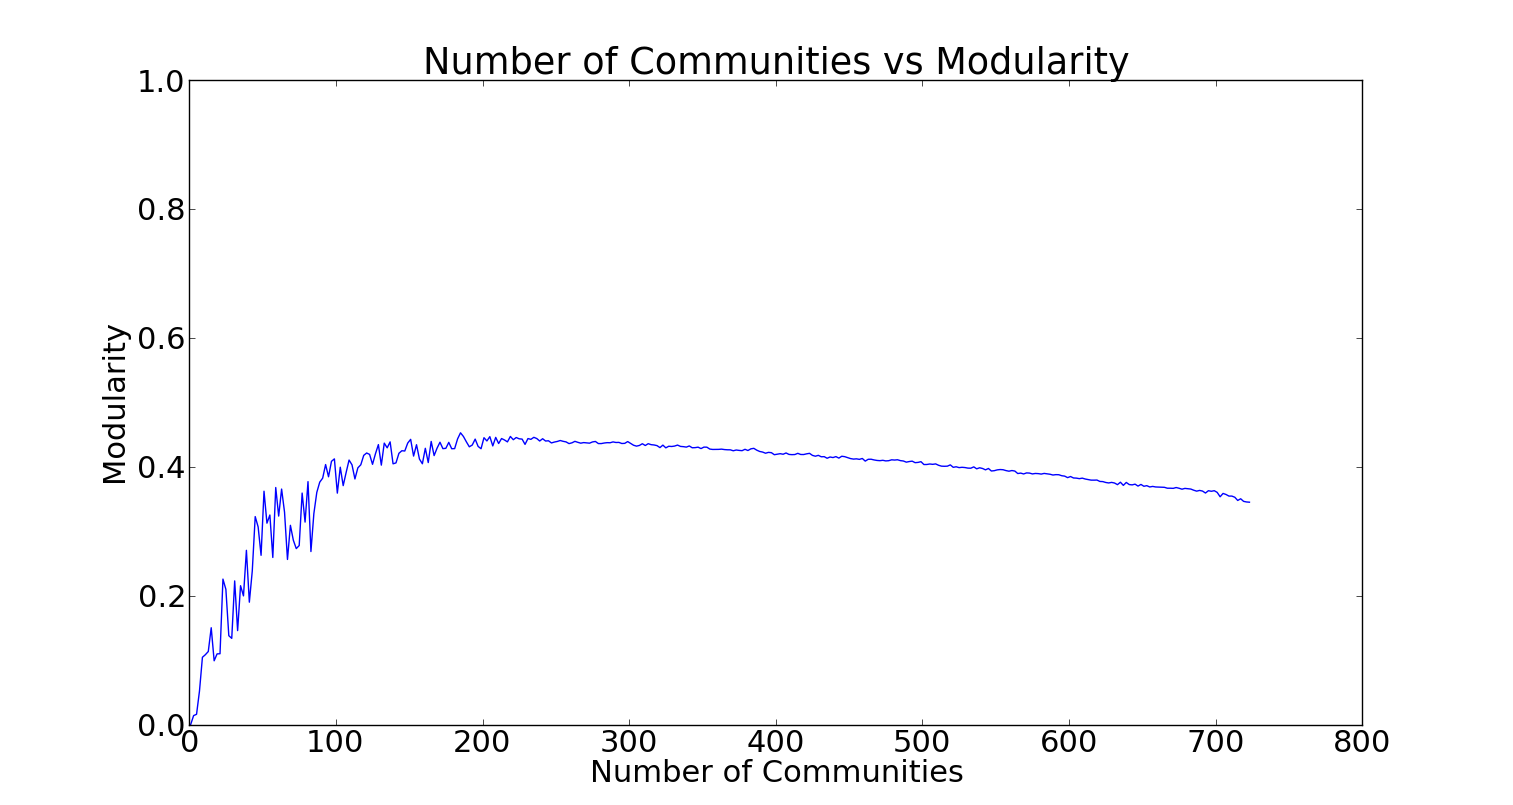
\includegraphics[width=.8\linewidth]{modularityf12.png}
  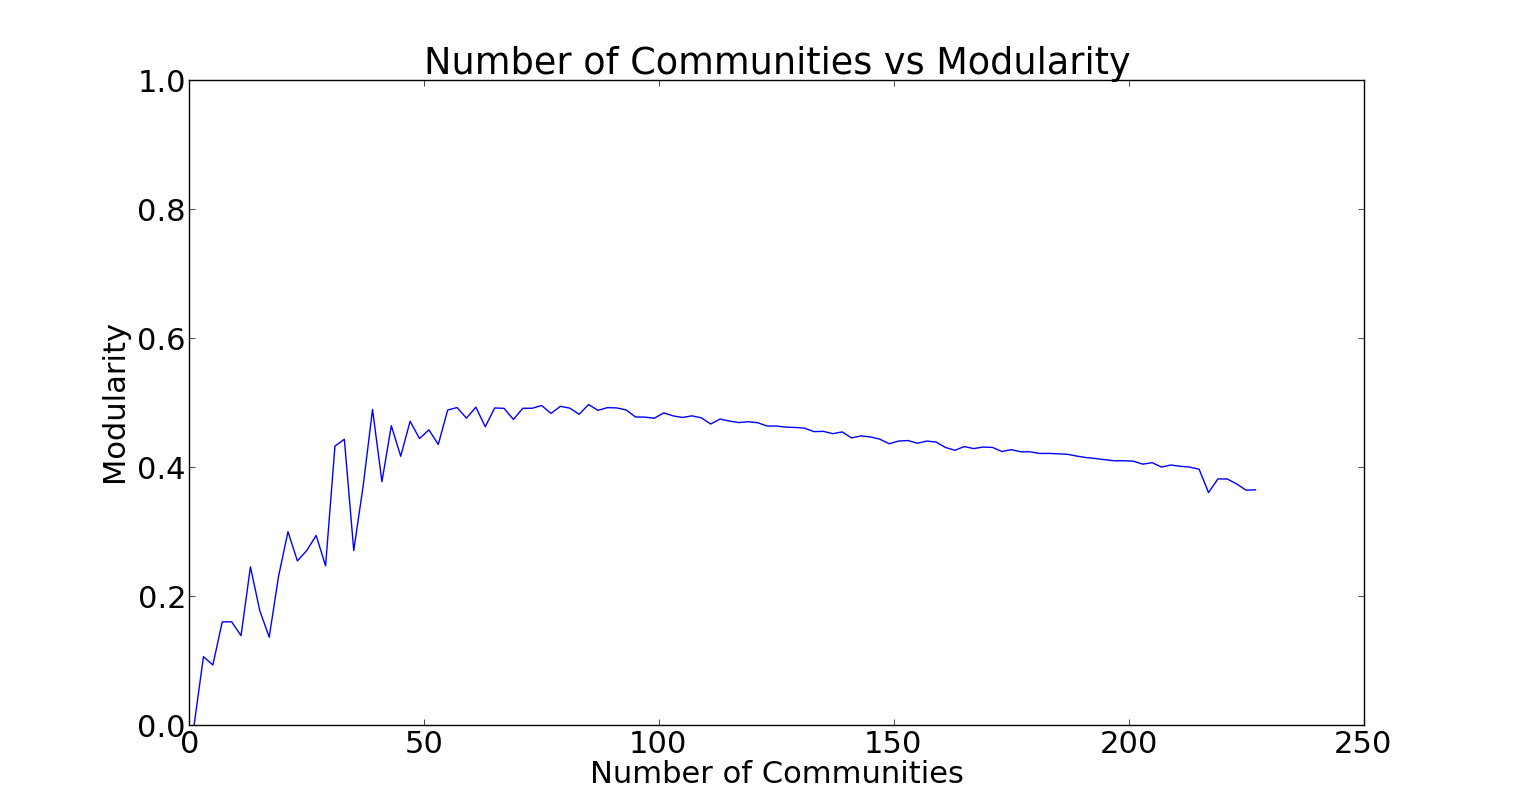
\includegraphics[width=.8\linewidth]{modularitys13.png}
  \caption{Number of Communities vs Modularity. 6.002x Fall 2012 is on top and 6.002x Spring 2013 is on bottom}
  \label{modularity}
\end{figure}



Unlike Louvain Method, spectral clustering requires the number of communities in order to produce a result. The result we present in Table \ref{results} show the number of clusters that achieves the highest modularity. Figure \ref{modularity} shows how the number of communities specified affects the modularity of interaction graph for 6.002x Fall 2012. 



% \begin{figure}[!htb]
%     \centering
%     \caption{Best Spectral Partition for 6.002x Spring 2012}
%     \label{spectral_best}
% \end{figure}

% \begin{figure}[!htb]
%     \centering
%     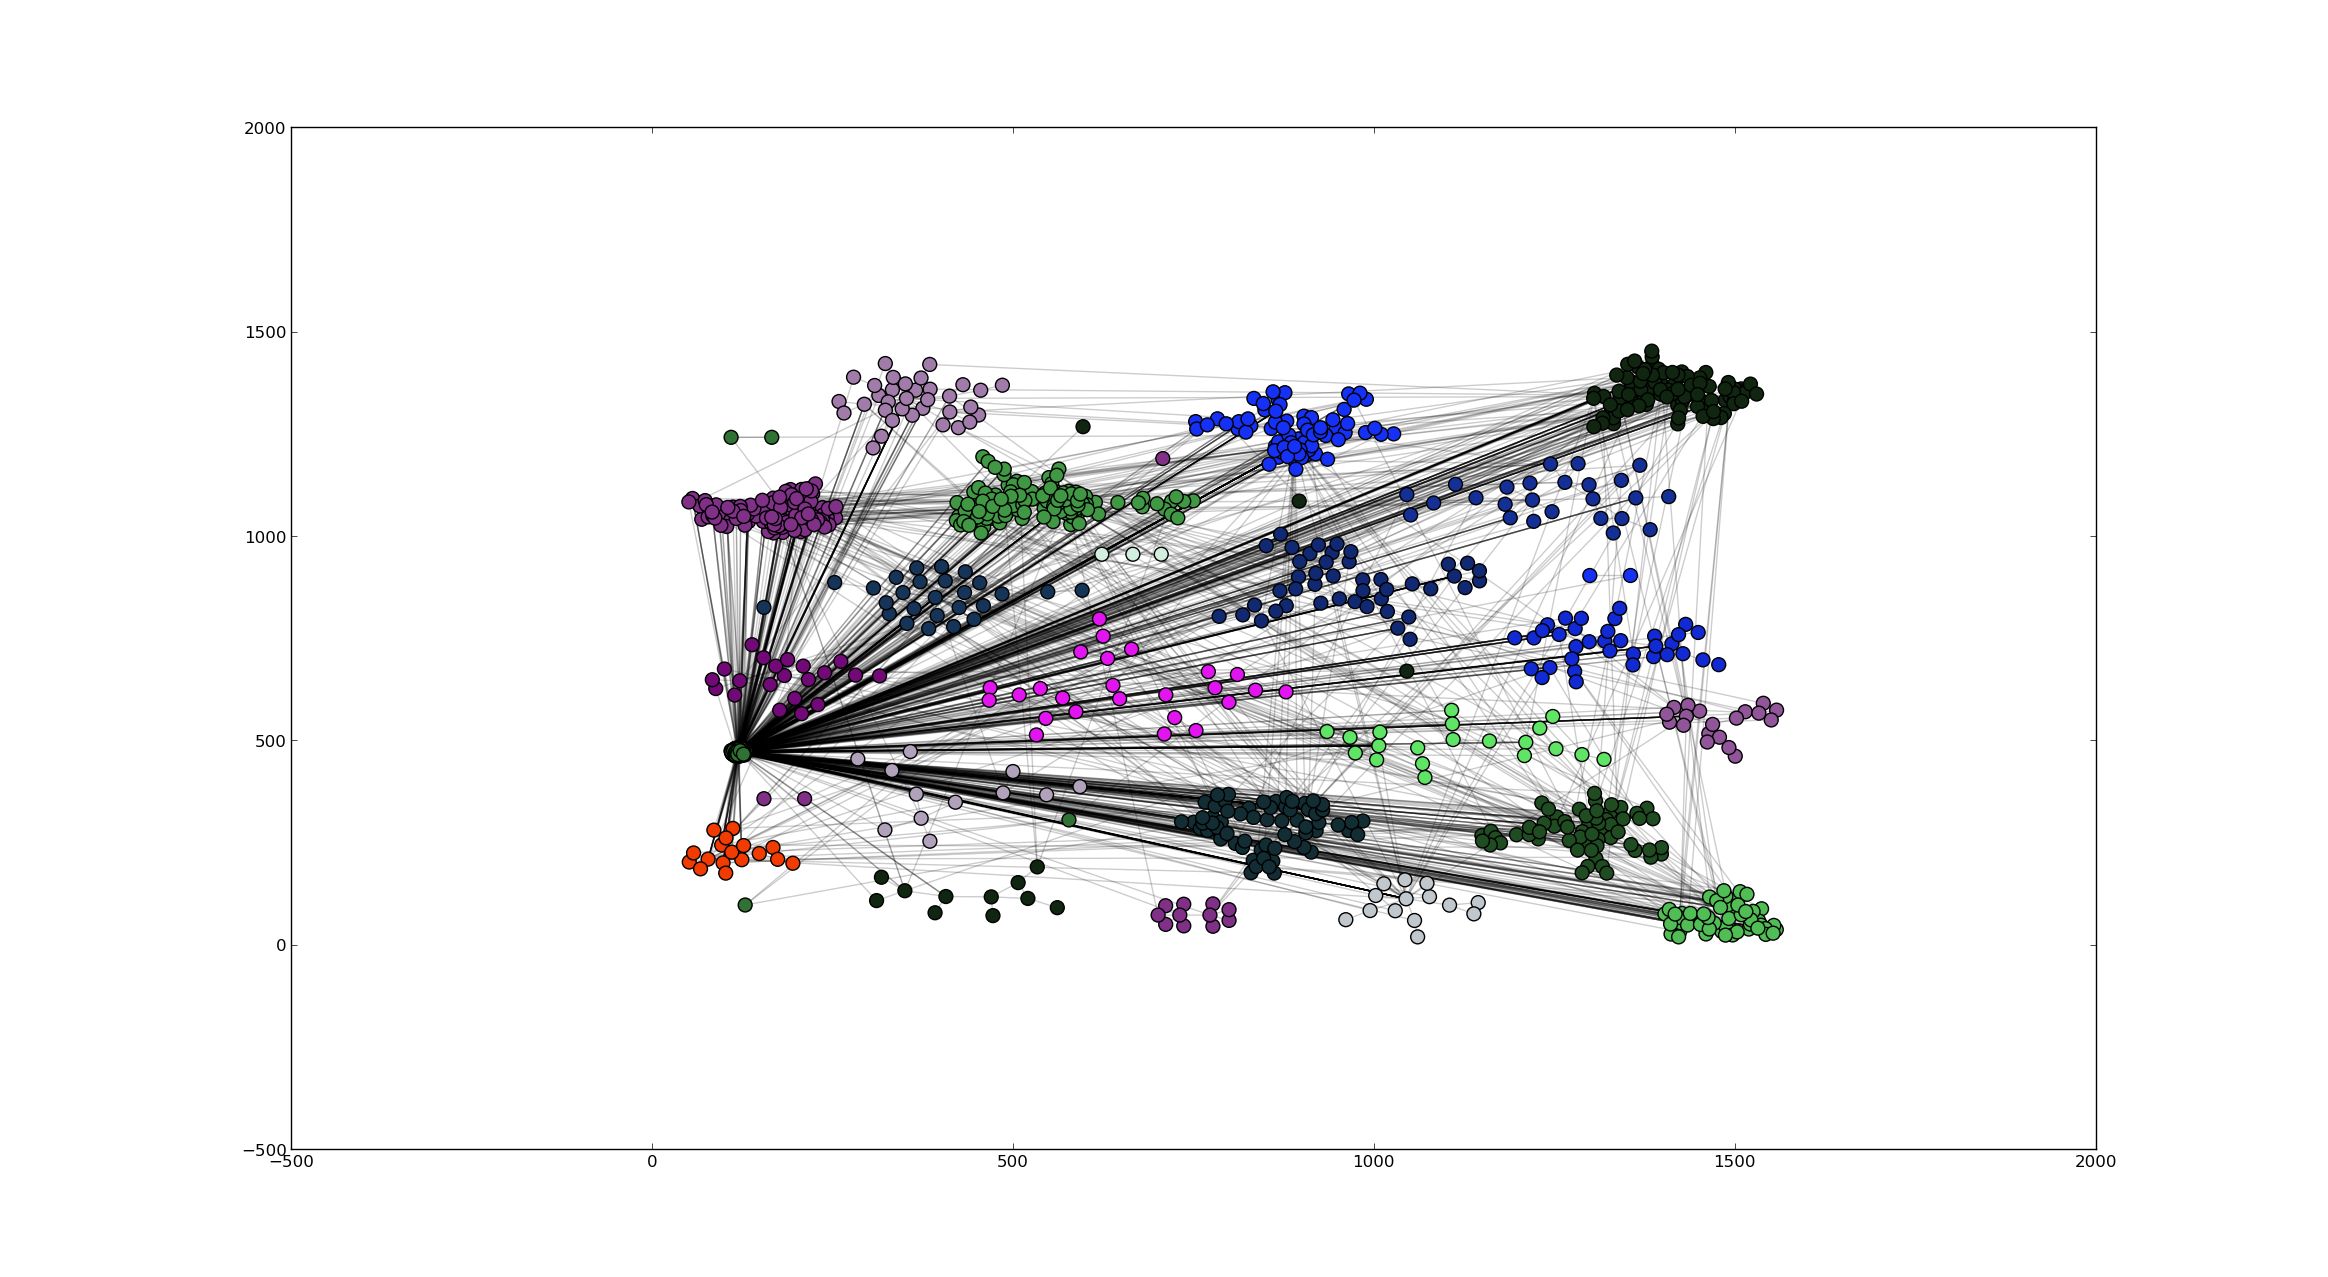
\includegraphics[width=.8\linewidth]{spectral_22.png}
%     \caption{Spectral Partition with 22 communities for 6.002x Spring 2012}
%     \label{spectral_22}
% \end{figure}




